
\documentclass[UTF8]{beamer}
\usetheme{Copenhagen}
%\usepackage{subfigure}
\usepackage{url}   % 网页链接
\usepackage{subcaption}
\usepackage{epstopdf}
\usepackage{graphicx}
\usepackage{booktabs}
%\usepackage[ruled,linesnumbered]{algorithm2e}
%\usepackage[space,space,hyperref]{ctex}
\usepackage{ctex} %可以改成中文版

\captionsetup{font={small}}
\AtBeginSection[]{
	\begin{frame}
		\vfill
		\centering
		\begin{beamercolorbox}[sep=10pt,center,shadow=true,rounded=true]{title}
			\usebeamerfont{title}\insertsectionhead\par%
		\end{beamercolorbox}
		\vfill
	\end{frame}
}

\AtBeginSubsection[]{
	\begin{frame}
	%	\vfill
		\centering
		\begin{beamercolorbox}[sep=6pt,center,shadow=true]{title}
			\usebeamerfont{title}\insertsubsectionhead\par%
		\end{beamercolorbox}
	%	\vfill
	\end{frame}
}
\usetheme{Warsaw}
\colorlet{beamer@blendedblue}{green!30!black}
\author{答辩人: 吴茼17307053\quad 指导老师: 李嘉}
\title{层叠成像中的相位恢复问题}
\institute{中山大学数学学院\quad 数学与应用数学专业}
\titlegraphic{
\includegraphics[height=1.5cm]{SYSULogo}}
\setbeamertemplate{headline}{}
\begin{document}

\frame{\titlepage}

\begin{frame} \frametitle{Contents}
%\framesubtitle{Acknowledgment: this slide is based on Prof. Wen's and Dr. Stefano's lecture notes.}
\tableofcontents
\end{frame}

\section{研究背景}


\begin{frame} \frametitle{Introduction}
\begin{figure}[H]
\centering

    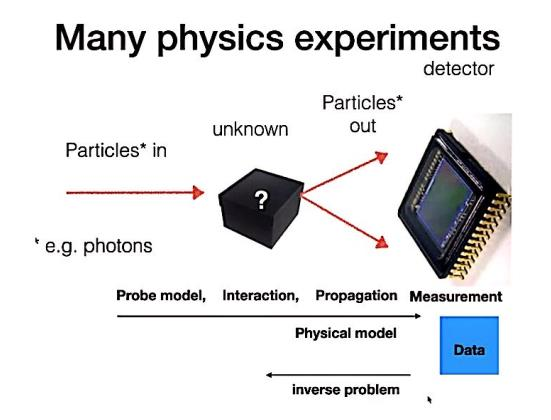
\includegraphics[width=1\linewidth]{../figures0/overall.jpg}  
   
\end{figure}
\end{frame}

\begin{frame} \frametitle{Missing phase problem}
\begin{figure}[H]
\centering

    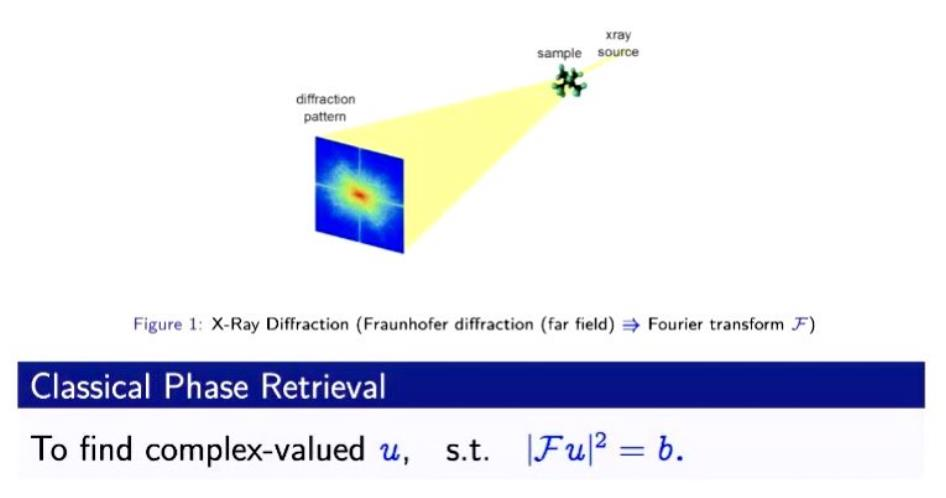
\includegraphics[width=1\linewidth]{../figures0/problem.jpg}  
   
\end{figure}
\end{frame}






\subsection{层叠成像}


%Here


%The theorem above serves as a benchmark result, but using Gaussian vectors as measurement vectors $a_k$ is not very realistic. For practical purposes, we prefer sets of measurement vectors that obey certain diffraction structure. 
%For practical purposes, we may prefer sets of measurement vectors that %obey certain diffraction structure. 


\begin{frame}[c]\frametitle{Ptychographic Phase Retrieval}
\begin{equation}
\label{basic}
f_{j}=\left|\mathcal{F}\left( \mathcal{S}_{j} u  \circ \omega \right)\right|
\end{equation}

In a discrete setting, $u \in \mathbb{C}^{n^2}$ is a 2D image with $n \times n$ pixels, $\omega \in \mathbb{C}^{m^2}$ is a localized 2D probe with $m \times m$ pixels.

$f_{j} \in \mathbb{R}_{+}^{m^2}(\forall 1 \leq j \leq K)$ is a stack of phaseless measurements. Here $|\cdot|$ represents the element-wise absolute value of a vector, o denotes the elementwise multiplication, and $\mathcal{F}$ denotes the normalized 2 dimensional discrete Fourier transform. Each $\mathcal{S}_{j} \in \mathbb{R}^{m^2 \times n^2}$ is a binary matrix that crops a region $j$ of size $m^2$ from the image $u$.


\end{frame}


\begin{frame}[c]\frametitle{Ptychographic Phase Retrieval}
\begin{figure}[H]
	\centering
	
	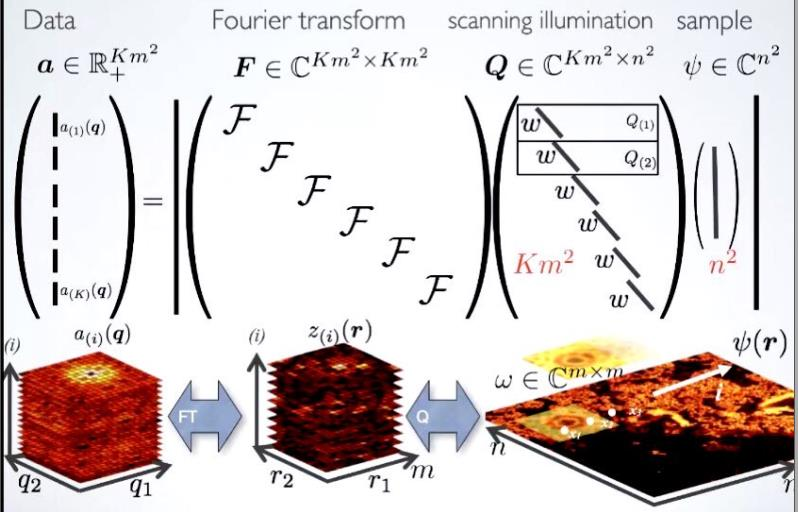
\includegraphics[width=1\linewidth]{../figures0/ptycho.jpg}  
	
\end{figure}

\end{frame}




\section{偏向干层叠成像}
\begin{frame}[c]\frametitle{New problem: partially coherent}

\begin{figure}
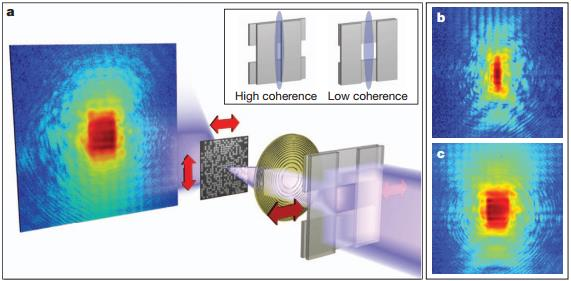
\includegraphics[width=1\linewidth]{../figures0/partially.jpg}  
  \end{figure}
\end{frame}

\subsection{模型}
\begin{frame} \frametitle{Target model: phobe vibration}
	
	Continuous setting:
	
	\begin{equation}
	f_{p c, j}(q) = \int\left|\mathcal{F}_{x \rightarrow q}\left(\mathcal{S}_{j} u(x) \omega(x-y)\right)\right|^{2} \kappa(y) \mathrm{d} y
	\end{equation}
	
	Discrete setting:
	
	\begin{equation}
	f_{p c, j}=\sum_{i} \kappa_{i}\left|\mathcal{F}\left( \mathcal{S}_{j} u \circ \left(\mathcal{T}_{i} \omega\right) \right)\right|^{2}
	\label{model:target}
	\end{equation}
	

\end{frame}


\begin{frame}[c]\frametitle{Density matrix}
$$
\begin{small}
\begin{aligned}
&f_{p c, j}(q) = \int\left|\mathcal{F}_{x \rightarrow q}\left(\mathcal{S}_{j} u(x) \omega(x-y)\right)\right|^{2} \kappa(y) \mathrm{d} y\\
& = \int\int  
\mathcal{S}_{j} u(x_1)e^{-iqx_1} \omega(x_1-y)  \overline{ \mathcal{S}_{j} u(x_2)e^{-iqx_2} \omega(x_2-y) }   \int   \kappa(y)   dy
dx_1 dx_2 \\
& = \int\int  
\mathcal{S}_{j} u(x_1)e^{-iqx_1}  \overline{ \mathcal{S}_{j} u(x_2)e^{-iqx_2}  }   (\int  \omega(x_1-y) \overline{\omega(x_2-y)} \kappa(y)   dy)
dx_1 dx_2 \\
\end{aligned}
\end{small}
$$	

Density matrix in time space:
\begin{equation}
\rho(x_1,x_2) = \int  \omega(x_1-y) \overline{\omega(x_2-y)} \kappa(y)   dy
\end{equation}

In discrete setting:

\begin{equation}
\rho = \sum_i \hat{w}_i \hat{w}_i^*, \hat{w}_i = \sqrt{\kappa_{i}}\mathcal{T}_{i} \omega
\end{equation}

\end{frame}

\begin{frame}[c]
	
	\begin{small}
	$$
		\begin{aligned}
		&f_{p c, j}(q) = \int\left|\mathcal{F}_{x \rightarrow q}\left(\mathcal{S}_{j} u(x) \omega(x-y)\right)\right|^{2} \kappa(y) \mathrm{d} y\\
		&= \int \int \mathcal{S}_{j} u(x_1) \omega(x_1-y) e^{-iqx_1} dx_1 \overline{ \int \mathcal{S}_{j} u(x_2) \omega(x_2-y) e^{-iqx_2}dx_2 }  \kappa(y)   dy \\
		&= \int \int \widehat{\mathcal{S}_{j} u(x_1)e^{-iqx_1}} \widehat{\omega(x_1-y)}  dx_1' \overline{ \int \widehat{(\mathcal{S}_{j}u)(x_2) e^{-iqx_2} }  \widehat{\omega(x_2-y)} dx_2' } \kappa(y)   dy\\
		& = \int\int  
		\widehat{\mathcal{S}_{j} u(x_1)e^{-iqx_1}} \widehat{\omega}(x_1')e^{-iyx_1'}  \overline{ \widehat{\mathcal{S}_{j} u(x_2)e^{-iqx_2}} \widehat{\omega}(x_2')e^{-iyx_2'} }   \int   \kappa(y)   dy
		dx_1' dx_2' \\
		& =  \int\int  
		\widehat{(\mathcal{S}_{j}u)}(x_1' + q) \widehat{\omega}(x_1')   \overline{ \widehat{(\mathcal{S}_{j}u)}(x_2' + q) \widehat{\omega}(x_2') }   (\int   \kappa(y)e^{-iy(x_1'-x_2')}  dy ) \\
		& = \int\int  
		\widehat{(\mathcal{S}_{j}u)}(x_1' + q)    \overline{ \widehat{(\mathcal{S}_{j}u)}(x_2' + q)  }    (\hat{\kappa}(x_1'-x_2')\widehat{\omega}(x_1') \overline{\widehat{\omega}(x_2')}) 
		dx_1' dx_2'
		\end{aligned}
	$$	
	\end{small}
	
	
	
\end{frame}

\begin{frame}
	Density matrix in Fourier space:
	\begin{equation}
		\widehat{\rho}(x_1',x_2') = \int\int \rho(x_1,x_2) e^{-i x_1x_1'} e^{-i x_2 x_2'}dx_1'dx_2'= \hat{\kappa}(x_1'-x_2')\widehat{\omega}(x_1') \overline{\widehat{\omega}(x_2')}
	\end{equation}

	
	
	In discrete setting:
	
	\begin{equation}
		\hat{\rho} = F \rho F^* = \hat{\kappa} .* (\hat{\omega} \hat{\omega}^*)
	\end{equation}
$\rho$ is psd, and so is $\hat{\rho}$. Use truncated SVD to get a low-rank approximation:
$$
\rho \approx \sum_{k=1}^{r} w_k w_k^* 
$$
\end{frame}



\begin{frame}[c]\frametitle{General model}
\framesubtitle{Thibault, Pierre, and Andreas Menzel. "Reconstructing state mixtures from diffraction measurements." Nature 494.7435 (2013): 68-71.}



\structure{Blind ptychography model + quantum state tomography.}

Phobe $w$ is assumed to be in mixed state to represent partially coherent effect.

\begin{equation}
\label{model:sep} 
\begin{aligned}
&\mbox{Find } u, r \mbox{ $w_k$   }s.t. \\
&f_{p c, j}=\sum_{k=1}^r \left|\mathcal{F}\left( \mathcal{S}_{j} u \circ \left(\omega_k\right) \right)\right|^{2}  
\end{aligned}
\end{equation}
\end{frame}










\subsection{算法}
\begin{frame}[c]\frametitle{Ptychographic Phase Retrieval}
	
	\begin{enumerate}
		\item optimization problem
		$$
		\min \rho(u,\omega):=\sum_{j=1}^{K}  \frac{1}{2}\left\|  \sqrt { \sum_{i=1}^{r} \left|\mathcal{F} ( \mathcal{S}_{j} u  \circ \omega_i) \right| }-f_{j}\right\|_{2}^{2}
		$$
		\item Reformulation:
		$
		\min \sum_{j=1}^{K} \frac{1}{2}\left\| \sqrt{ \sum_{i=1}^r \left|z_{j,i}\right| }-f_{j}\right\|_{2}^{2} 
		$
		\begin{small}
				$
			\text {, s.t. } z_{j,i}= \mathcal{A}_{j}(\omega_i, u):=\mathcal{F}\left(\omega_i \circ \mathcal{S}_{j} u\right),j=1... K
			$
		\end{small}
	
	
		
		
		\item Combine
		\begin{footnotesize}
		 $z_i = \mathcal{A}(\omega_i, u) := \left(\mathcal{A}_{1}^{T}(\omega_i, u), \mathcal{A}_{2}^{T}(\omega_i, u),..., \mathcal{A}_{K}^{T}(\omega_i, u)\right)^{T} 
			\in \mathbb{C}^{ Km^2}$,
			
			$f := (f_1^T,f_2^T, \ldots, f_K^T)^T$;
			$z = (z_1^T,z_2^T,...,z_r^T)^T \in \mathbb{C}^{ Krm^2}$
		\end{footnotesize}
	    \begin{small}
	    		$$
	    	\min \mathcal{G}(z) := \frac{1}{2}\left\| \sqrt{ \sum_{i=1}^r \left|z_{i}\right| } -f\right\|_{2}^{2} \text {, s.t. } z_i= \mathcal{A}(\omega_i, u), i = 1,...,r
	    	$$
	    \end{small}
	
		
	\end{enumerate}
	
	
\end{frame}

\begin{frame}[c]\frametitle{ADMM(Alternating Direction Method Of Multipliers)}
\begin{equation}
\begin{aligned}
&\min _{\omega, u, z} \mathcal{G}(z)+\mathbb{I}_{\mathcal{X}_{1}}(\omega)+\mathbb{I}_{\mathcal{X}_{2}}(u)
+ \mathbb{I}_{\mathcal{X}_{3}}(D\alpha) \\
&s.t. \quad z-\mathcal{A}(\omega, u)=0, \quad \Omega(D\alpha) - \omega = 0. \\
\end{aligned}
\end{equation}

The corresponding augmented Lagrangian reads
$$
\begin{aligned}
\Upsilon_{\beta}(\omega, u, z, \Lambda,D,\alpha,\Lambda_2):=&\mathcal{G}(z)+\mathbb{I}_{\mathcal{X}_{1}}(\omega)+\mathbb{I}_{\mathcal{X}_{2}}(u) + \mathbb{I}_{\mathcal{X}_{3}}(D)\\
+&\Re(\langle z-\mathcal{A}(\omega, u), \Lambda\rangle)+\frac{\beta}{2}\|z-\mathcal{A}(\omega, u)\|^{2}
\\
+&\Re(\langle \Omega(D\alpha) - \omega, \Lambda_2\rangle)+\frac{\beta_2}{2}\| \Omega(D\alpha) - \omega\|^{2}
\end{aligned}
$$
	
\end{frame}
\begin{frame}
\begin{align}
\text { Step 1: } & \omega^{k+1}=\arg \min _{\omega} \frac{\beta}{2}\|z-\mathcal{A}(\omega, u) + \Lambda \|^{2} +\\
&\frac{\beta_{2}}{2}||\omega - (\Omega(D^k\alpha^k) + \Lambda_2)||^2 + 
\frac{\alpha_{1}}{2}\left\|\omega-\omega^{k}\right\|_{M_{1}^{k}}^{2}, \notag \\
\text { Step 2: } & u^{k+1}=\arg \min _{u} \frac{\beta}{2}\|z-\mathcal{A}(\omega, u) + \Lambda \|^{2} +\frac{\alpha_{2}}{2}\left\|u-u^{k}\right\|_{M_{2}^{k}}^{2}, \notag \\ \text { Step 3: } & z^{k+1}=\arg \min _{z} \frac{\beta}{2}\|z-\mathcal{A}(\omega, u) + \Lambda \|^{2} , \notag \\
\text { Step 4: } & D^{k+1}=\arg \min _{D} \mathbb{I}_{\mathcal{X}_{3}}(D\alpha) +
\frac{\beta_2}{2}\| \Omega(D^k\alpha^k) - \omega^{k+1}\|^{2} \notag \\
\text { Step 5: } & \alpha^{k+1}=\arg \min _{\alpha}  \frac{\beta_2}{2}\| \Omega(D^{k+1}\alpha^k) - \omega^{k+1}\|^{2}\notag \\
\text { Step 6: } &
\Lambda^{k+1}=\Lambda^{k}+\left(z^{k+1}-\mathcal{A}\left(\omega^{k+1}, u^{k+1}\right)\right)  \label{Lup}\\
\text { Step 7: } & \Lambda_2^{k+1}=\Lambda_2^{k}+ (\Omega(D^{k+1}\alpha^{k+1}) - \omega^{k+1}) \label{L2up}
\end{align}
\end{frame}

\begin{frame}[c]\frametitle{Subproblems $\omega$ and $u$ }
	$$
	\begin{aligned}
	&\omega^{k+1}=\arg \min _{\omega \in \mathcal{X}_{1}} \frac{1}{2}\left\|z^{k} + \Lambda^k -\mathcal{A}\left(\omega, u^{k}\right)\right\|^{2}\\
	&=\arg \min _{\omega \in \mathcal{X}_{1}} \frac{1}{2}\left\|\hat{z}^{k}-\mathcal{A}\left(\omega, u^{k}\right)\right\|^{2}\\
	\end{aligned}
	$$
	The close form solution of Step 1 is given as:
\begin{equation}
\omega^{k+1}=\operatorname{Proj}\left(\frac{ \beta\sum_{j}\left(\mathcal{S}_{j} u^{k}\right)^{*} \circ [ \left(\mathcal{F}^{-1} \hat{z}^k\right)(:,:,j,:) ]
	+ \beta_2 \hat{\Omega}^k}{ \beta \sum_{j}\left|\mathcal{S}_{j} u^{k}\right|^{2}+\beta_2} ; \mathcal{X}_{1}\right)
\label{omegaup}
\end{equation}
\begin{equation}
\begin{aligned}
	&\quad u^{k+1}=\operatorname{Proj}\left(\frac{\sum_{j,i} \mathcal{S}_{j}^{T}\left(\left(\omega_i^{k+1}\right)^{*} \circ \mathcal{F}^{-1} \hat{z}_{j,i}^{k}\right)}{\sum_{j,i}\left(\mathcal{S}_{j}^{T}\left|\omega_i^{k+1}\right|^{2}\right)} ; \mathcal{X}_{2}\right) \text { . }
\end{aligned}
\label{uup}
\end{equation}

	
\end{frame}

\begin{frame}[c]\frametitle{Subproblem $z$ }
$$
z^{k+1}=\arg \min _{z} \mathcal{G}(z)+\frac{\beta}{2}\left\|z-\mathcal{A}\left(\omega^{k+1}, u^{k+1}\right)+\Lambda^{k}\right\|^{2}
$$
$$
=\arg \min _{z} \frac{1}{2}|| \sqrt{ \sum_{i=1}^{r} |z(:,:,:,i)|^2} - Y||^2+\frac{\beta}{2}\left\|z - z^+\right\|^{2}
$$
where $z^+ = \mathcal{A}\left(\omega^{k+1}, u^{k+1}\right) - \Lambda^{k}$


The  close form solution of Step 3 is given as:
\begin{equation}
z_i^{k+1} = \dfrac{z_i^+ \dfrac{Y}{ M^k} + \beta z_i^+}{1+\beta}, 1 \leq i \leq r
\label{zup}
\end{equation}
where $z_i:= z(:,:,:,i)$ and $M^k =\sqrt{\sum_i |z_i^+|^2} \in \mathbb{C}^{px \times py \times K}$
\end{frame}



\begin{frame}[c]\frametitle{Subproblem $D$ and $\alpha$ }
$$
\begin{aligned}
D^{k+1} =& \arg \min_{D} \| \Omega -  w^{k+1} + \Lambda_2^{k}\|^{2} \\
=& \arg \min_{D} \| D\alpha^k - \hat {w}^{k+1}\|^{2} 
\end{aligned}
$$
where $\hat {w}^{k+1} = reshape( \omega^{k+1} - \Lambda_2^{k},[l,r])$,$D^*D=I$

The close form solution for $D^{k+1}$ is:
\begin{equation}
D^{k+1} = UV^*
\label{Dup}
\end{equation}
$$
\alpha^{k+1} = \arg \min_{\alpha} \| D^{k+1}\alpha - \hat {w}^{k+1}\|^{2} 
$$

The close form solution for $\alpha^{k+1}$ is:
\begin{equation}
\label{alpha up}
\alpha_i^{k+1} =  \sum_{i_0} \Re[ \overline{D^{k+1}(i_0,i)} \hat {w}^{k+1}(i_0,i) ]
(1\leq i \leq r)
\end{equation}
\end{frame}

%\begin{frame}
%\begin{algorithm}
%	%\SetAlgoRefName{} % no count number
%	\caption{ADMM for general mixed-state model\eqref{sep}}
%	\label{alg:admm}
%	\SetKwInOut{Ini}{Initialization}
%	\Ini{Set the number of states $r$, $\omega^{0}, u^{0}, z^{0}=\mathcal{A}\left(\omega^{0}, u^{0}\right), \Lambda^{0},\Lambda_2^{0}=0 $;\\
%		$D^0$ and $\alpha^0$ from SVD on $\omega^0$\\ maximum iteration number Iter $_{\text {Max }}$, and parameter $\beta$,$\beta_2$}
%	\KwOut{$u^{\star}:=u^{Iter_{M a x}}$ and $\omega^{\star}:=\omega^{ \operatorname{Iter}_{M a x}}$}
%	\For{$ii=0$ to $Iter _{M a x}-1$}{
%		Compute $\omega^{k+1}$ by \eqref{omegaup} with $\hat{z}^{k}:=z^{k}+\Lambda^{k}$ \;
%		Compute $u^{k+1}$  \eqref{uup}. with $\hat{z}^k$ the same as above\; 
%		Compute $z_i^{k+1}$,$1 \leq i \leq r$ by \eqref{zup}. with $z^+ = \mathcal{A}\left(\omega^{k+1}, u^{k+1}\right) - \Lambda^{k}$\;
%		Compute $D^{k+1}$ \eqref{Dup}. \;
%		Compute $\alpha_i,1 \leq i \leq r$ \eqref{alpha up}.  \;
%		Update the multiplier as Step 6 and Step 7 of \eqref{Lup} and \eqref{L2up}\;
%	}
%\end{algorithm}
%
%\end{frame}

\subsection{数值实验}

\begin{frame} \frametitle{Experiment setting}


	\begin{center}
		\resizebox{\textwidth}{!}{
			\begin{tabular}{ccc}
				\toprule
				Parameters & Illustration & Values \\
				\hline
				$N_x,N_y$ & size of image $u$ & 128,128  \\
				\hline
				$p_x,p_y$ & size of phobe $w$ &  64,64\\
				
				\hline
				$Dist$ & scan distance between  neighborhood frames &  4,8,16\\
				\hline
				$N$ & number of frames in diffusion image stacks &   \\ 
				\hline
				$r$ & number of states(modes) & 1(coherent) to 15 \\
				\hline
				gridFlag & types of scan methods & 1(rectangular lattice),\\
				& &2(hexagonal),3(randomly disturb on 2)  \\
				\hline
				blurFlag & types of partially coherent effect & 1 ,2\eqref{model:target}\\
				\bottomrule 
			\end{tabular}
		}
	\end{center}

\end{frame}


\begin{frame} \frametitle{Performance Metrics}

\begin{enumerate}
\item Relative error $err$ and signal-to-noise ratio $snr$
$$
err^k = \dfrac{|| c u^k - u_{true} ||_F  }{||c u^k||_F}, c = \frac{sum(u_{true} \circ \overline{u^k}) }{||u^k||_F^2}
$$
$$
snr^k = -20\log_{10}(err^k)
$$
 $c$ is an estimated scale factor
 
 %and $sum$ means the sum of all elements in the target matrix. 

\item R-factor $R$

Let $zz = \mathcal{A}_{j}\left(\omega^{k}, u^{k}\right)$
$$
R^{k}:=\frac{\left\| |zz|-f\right\|_{1}}{\|f\|_{1}}
$$

%$R$ measures the difference between the reconstruction diffraction stacks and groundtruth stacks $f$. 

%We don't always know $u_{true}$, $Y$ is the only input data for our algorithm, and R-factor can be used to verify the convergence.

%\item signal-to-noise ratio $SNR$
%$$
%SNR^k = -20\log_{10} (\dfrac{|| u^k - u_{true} ||_F  }{|| u_{true}||_F})
%$$


\end{enumerate} 
\end{frame}


\begin{frame} \frametitle{Simulation Experiment}

%$Dist=8$, regular grid, viberation model, and $\kappa$ is a guassian kernel with $\sigma = (15,15)$. $\beta=0.05$ is chosen as algorithm parameter for ADMM.

\begin{figure}
\centering
\begin{subfigure}{\textwidth}
    \centering
    % include first image
    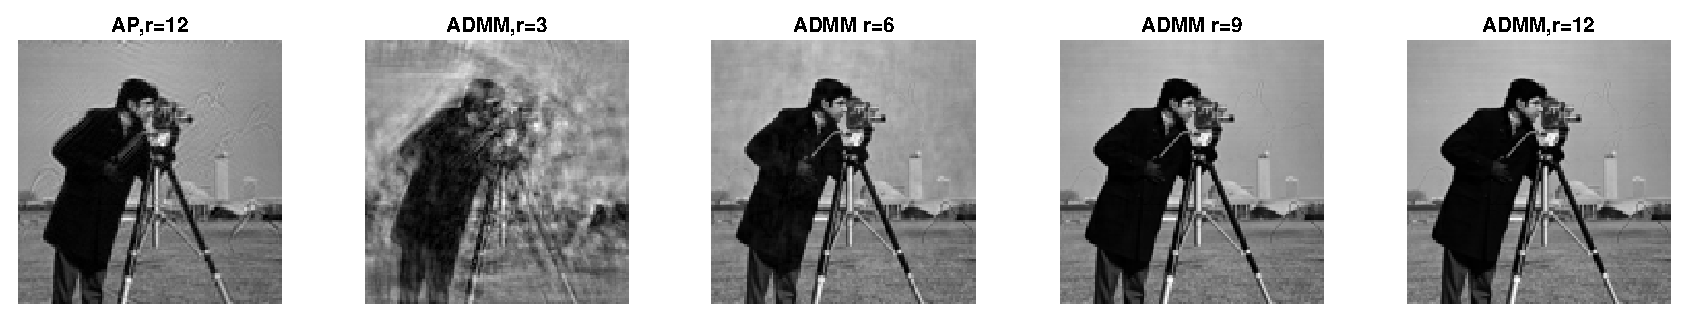
\includegraphics[width=0.9\linewidth]{../figures/modes_u.eps}  
   \caption{Amplitude}
    \label{fig:modes_u}
 \end{subfigure}
 \begin{subfigure}{1\textwidth}
    \centering
    % include second image
    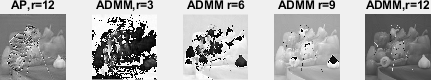
\includegraphics[width=.9\linewidth]{../figures/modes_u_phaze.png}  
    %\caption{Put your sub-caption here}
    \caption{Phase}
    \label{fig:modes_u_phaze}
 \end{subfigure}
 
    \label{fig:modes_images}

 \end{figure}


\end{frame}

\begin{frame} \frametitle{Simulation Experiment}
 \begin{figure}[H]
 \begin{subfigure}{.5\textwidth}
    \centering
    % include first image
    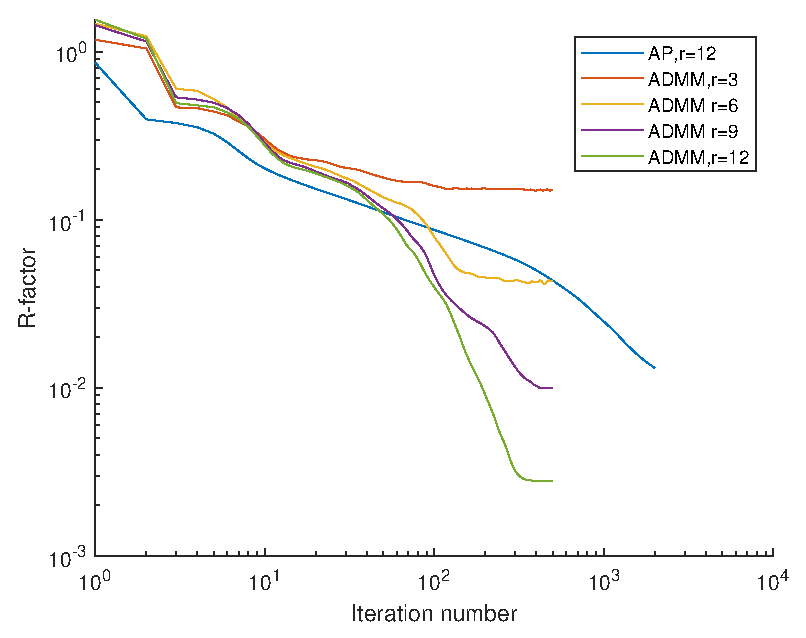
\includegraphics[width=1\linewidth]{../figures/modes_R.eps}  
    %\caption{}
    \label{fig:modes_R}
 \end{subfigure}
 \begin{subfigure}{.45\textwidth}
    \centering
    % include second image
    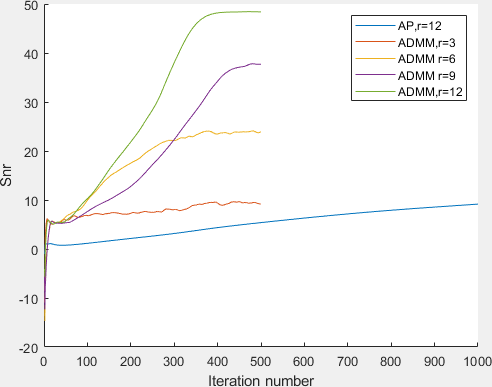
\includegraphics[width=1\linewidth]{../figures/modes_snr.png}  
    %\caption{Put your sub-caption here}
    \label{fig:modes_snr}
 \end{subfigure}
 \caption{R and snr. }
 \label{fig:noise}
 \end{figure}


%We first compare $snr$ and $R$ for reconstructed images using a different number of modes. When the number of modes increases, the $R-factor$ decreases, and the $snr$ increases. That indicates that the quality of the reconstructed image increases.

%The $R$ for 3,6,9,12 modes using ADMM algorithm are stable after 500 iterations at 0.15, 0.042, 0.0099, 0.0028, respectively, when $R$ for AP does not converge after 2000 iterations.

%similar k*f
\end{frame}

\begin{frame} \frametitle{Simulation Experiment}
\begin{figure}[H]
\centering
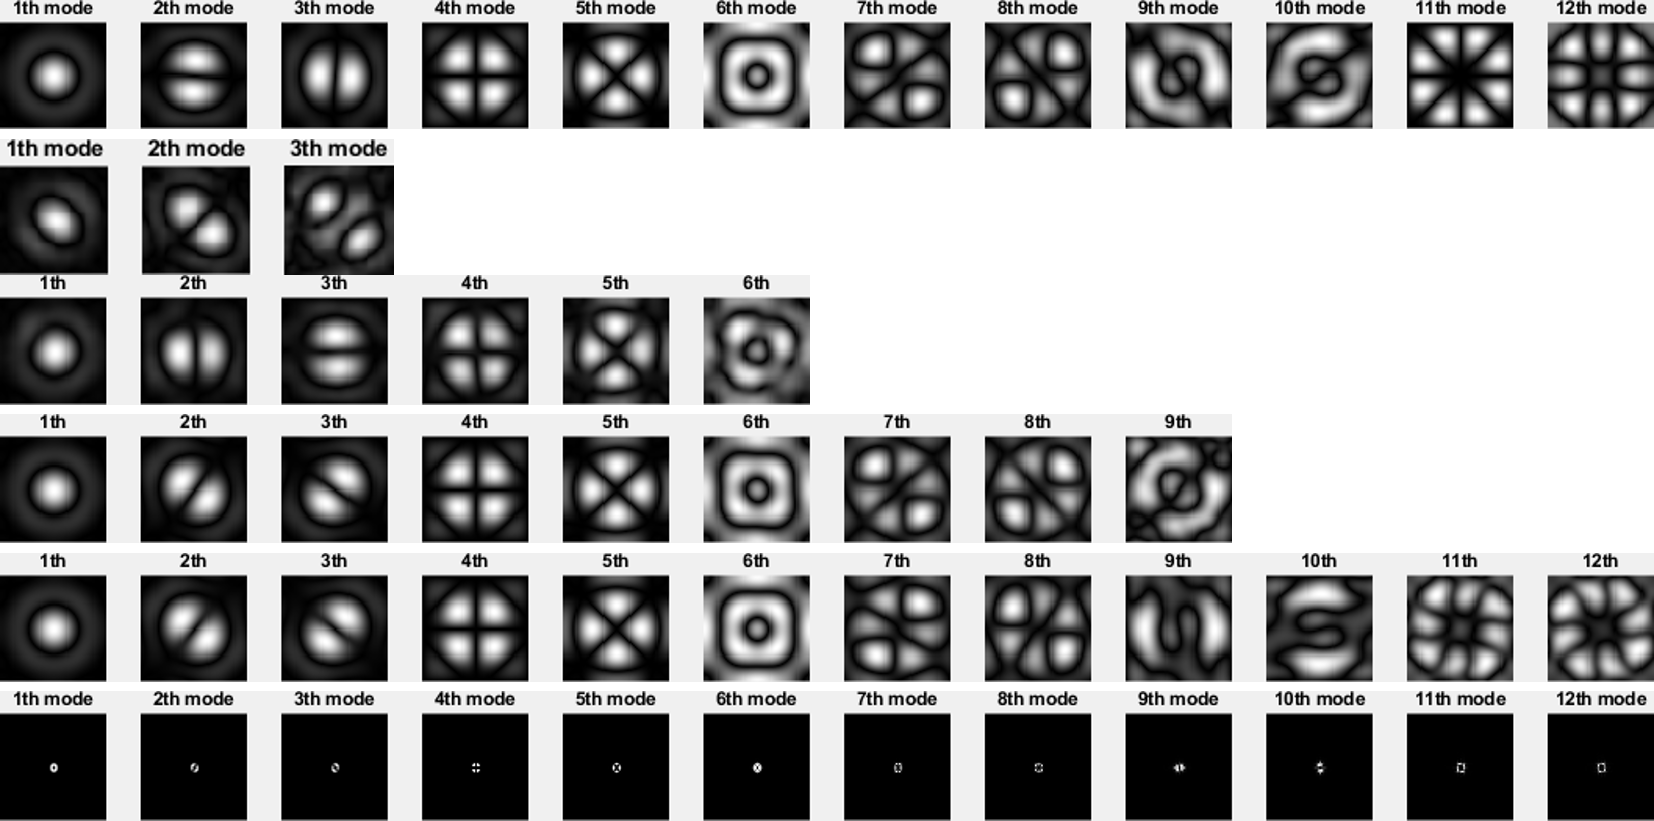
\includegraphics[width=1\linewidth]{../figures/modes_combine}
\caption{Mode pattern
	%. The first row represents the standard mode pattern. And the last two rows represent the mode pattern for 12 modes. Mode patterns are in the time domain except that the last row is in the frequency domain.
}
\label{fig:modescombine}
\end{figure}

%Standard mode pattern is obtained through performing SVD on standard density matrix generated from the model and extracting the first 12 modes. As shown in Figure \ref{fig:modescombine}, our algorithm can generally catch the main modes and get an optimal approximation.

\end{frame}

\begin{frame} \frametitle{Add the orthogonal constraint}
	%The experiment setting is the same as above except that we change $ratio=\beta_2\beta$ to introduce orthogonalization constraint in ADMM. The larger the $\beta_2$, the stricter the orthogonalization constraint. As a reference, we also tried performing orthogonalization as in Algorithm \ref{alg:ort} every 20 iterations. 
	%3
	\begin{figure}
		\begin{subfigure}{.33\textwidth}
			\centering
			% include first image
			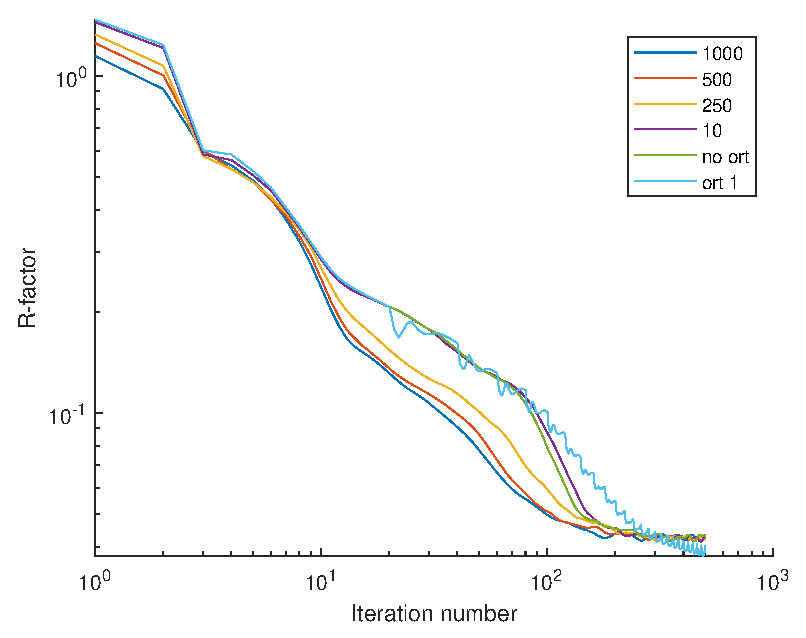
\includegraphics[width=1\linewidth]{../figures/ort_R.eps}  
			%\caption{}
			\label{fig:ort_R}
		\end{subfigure}
		\begin{subfigure}{.3\textwidth}
			\centering
			% include second image
			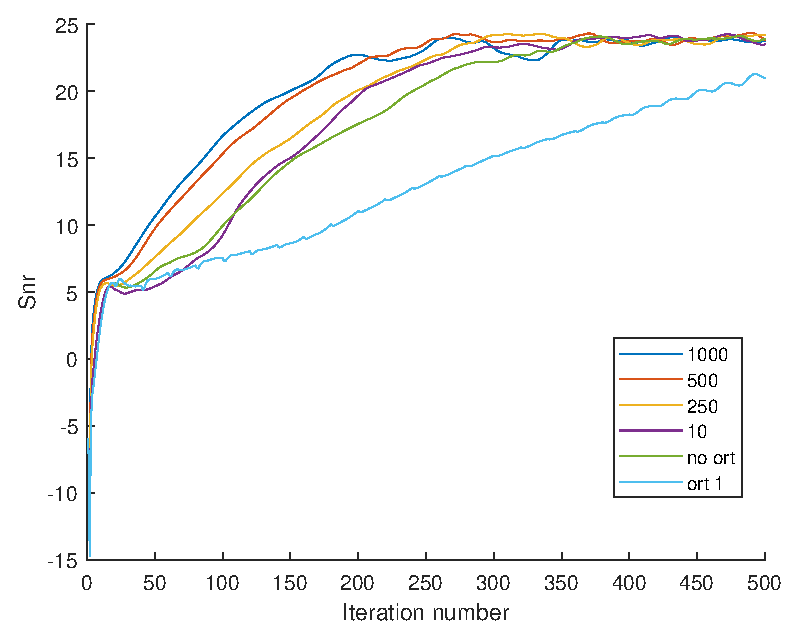
\includegraphics[width=1\linewidth]{../figures/ort_snr.eps}  
			%\caption{Put your sub-caption here}
			\label{fig:ort_snr}
		\end{subfigure}
		\begin{subfigure}{.3\textwidth}
			\centering
			% include second image
			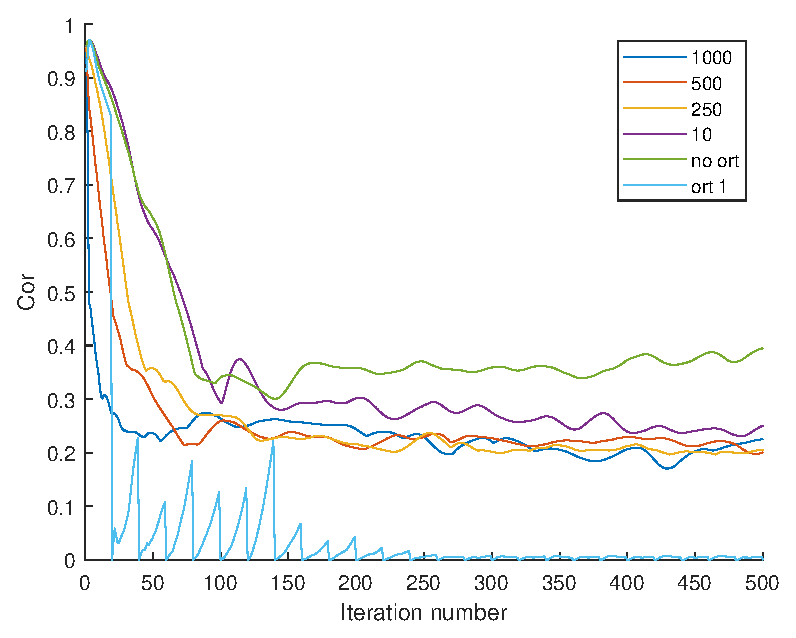
\includegraphics[width=1\linewidth]{../figures/ort_cor.eps}  
			%\caption{Put your sub-caption here}
			\label{fig:ort_cor}
		\end{subfigure}
		\caption{The vertical axis and horizontal axis are set in log-scale in the first subfigure for R-factor. The blue line represents $\beta_2/\beta=1000$ and works the best in this case. The green line represents the result without orthogonalization. 'ort 1' means performing orthogonalization every 20 iterations. }
		\label{fig:ort}
	\end{figure}
	
%	The reconstructed images are similar after 500 iterations, while $snr$ and $R factor$ using the ADMM algorithm with orthogonalization constraint improve faster. And the degree of correlation  $coherence$ between modes also decreases faster with larger $\beta_2$. 
	
\end{frame}

\section{总结和讨论}

\begin{frame} \frametitle{Conclusion}

\structure{主要贡献:}

验证了将目标模型放入通用模型框架下求解合理而且有效

\begin{enumerate}
\item 模型: 具体刻画了目标模型密度矩阵的结构,将
它放入通用模型的框架中

\item 算法: 改进了求解通用模型的相位恢复算法。
 将多模态 AP 改进为多模
态的 ADMM; 尝试在里面加入对不同模态的正交约束

\item 实验: 用模型生成仿真数据进行数值实验,并与传统 AP 的计算结果
和基于模型得到的“标准答案”进行对比,验证的算法的有效性
\end{enumerate}

\end{frame}

\begin{frame} \frametitle{Discussion}

\structure{不足:}	


 通用模型可以求解任何近似 $rank-r$ 的密
度矩阵,而我们目标模型中的密度矩阵结构更特殊:一个 toeplitz 矩阵与一个秩一
矩阵逐个元素相乘。没有利用到里面的特殊结构十分可惜。

$$
\widehat{\rho}(x_1',x_2') =  \hat{\kappa}(x_1'-x_2')\widehat{\omega}(x_1') \overline{\widehat{\omega}(x_2')}
$$


$$
\hat{\rho} = F \rho F^* = \hat{\kappa} .* (\hat{\omega} \hat{\omega}^*)
$$
	
\end{frame}

\begin{frame} \frametitle{Example: Guassian $\kappa$ (15 15)}
\begin{figure}[H]
\centering
%\caption{}
\begin{subfigure}{1\textwidth}
    \centering
    % include first image
    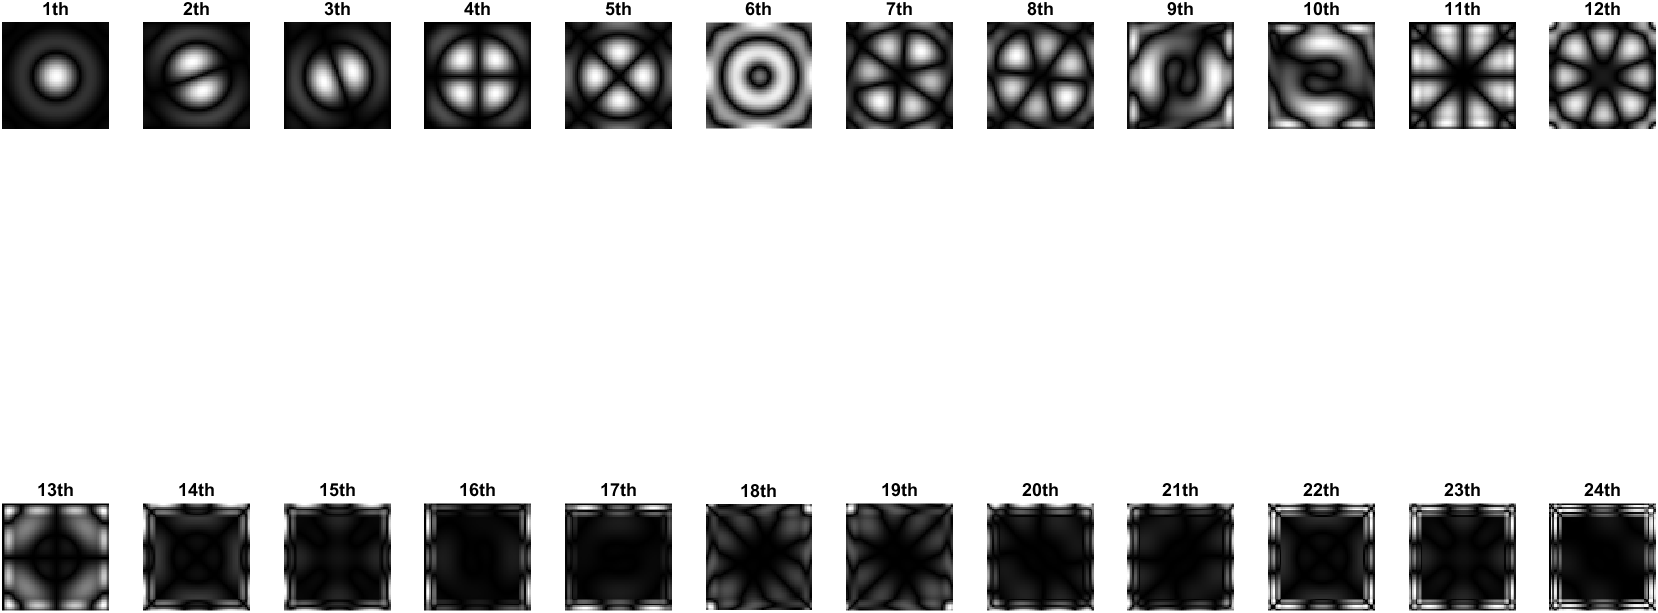
\includegraphics[width=0.8\linewidth]{../figures/ex_gu15_15.png}  
   %\caption{Ideal modes}
    \label{fig:modes_u}
 \end{subfigure}
 \begin{subfigure}{1\textwidth}
    \centering
    % include second image
    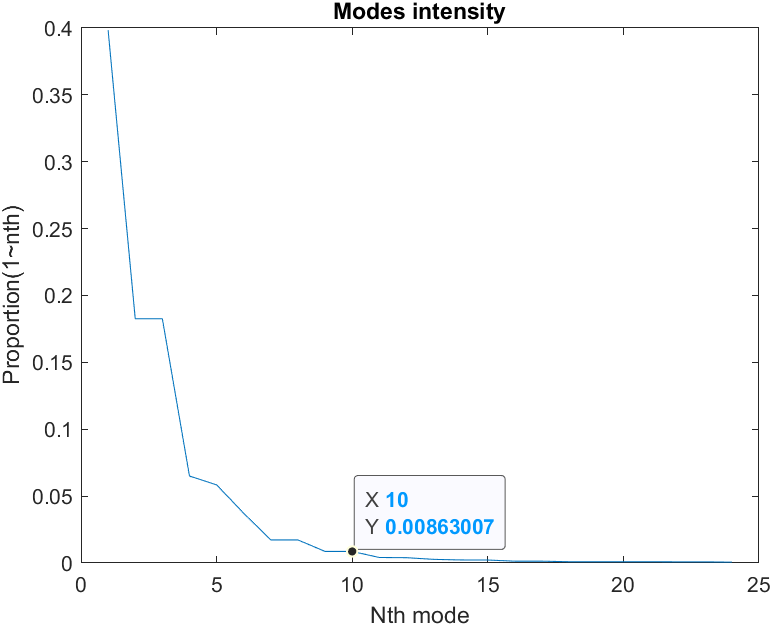
\includegraphics[width=.4\linewidth]{../figures/ex_gu15_15_s.png}  
    %\caption{Put your sub-caption here}
    %\caption{Singular value distribution}
    \label{fig:modes_u_phaze}
 \end{subfigure}
 
    \label{fig:modes_images}

 \end{figure}
\end{frame}


\begin{frame} \frametitle{Example: Retangular $\kappa$ (20 20)}
\begin{figure}[H]
\centering
\begin{subfigure}{1\textwidth}
    \centering
    % include first image
    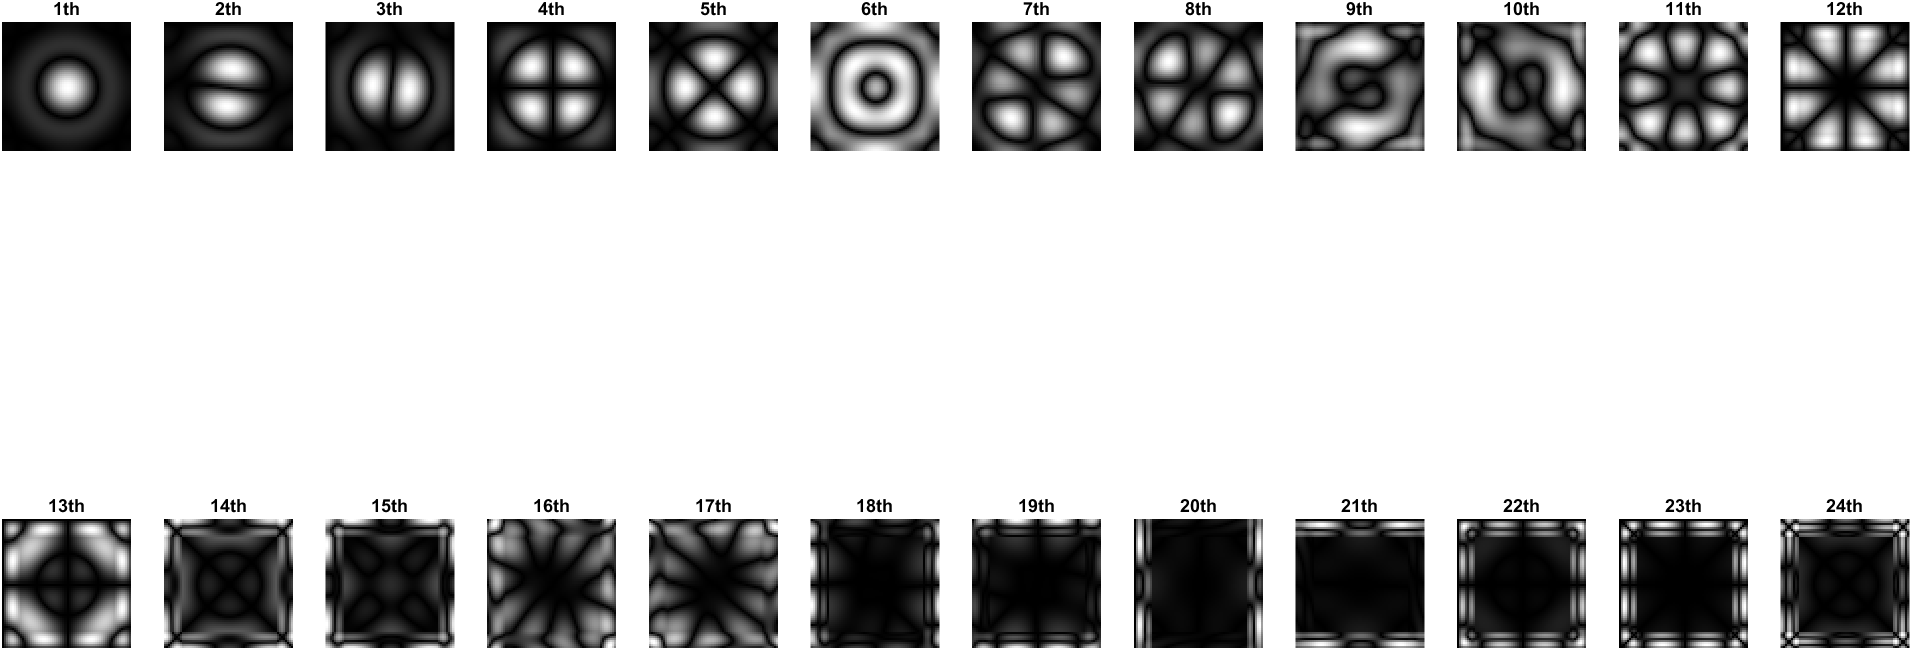
\includegraphics[width=0.8\linewidth]{../figures/ex_ave20.png}  
   %\caption{Ideal modes}
    \label{fig:modes_u}
 \end{subfigure}
 \begin{subfigure}{1\textwidth}
    \centering
    % include second image
    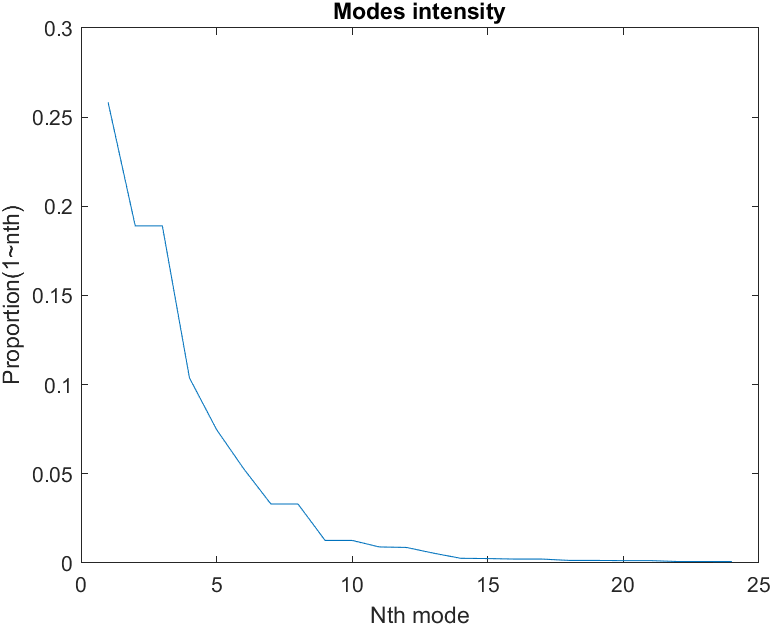
\includegraphics[width=.4\linewidth]{../figures/ex_ave20_s.png}  
    %\caption{Put your sub-caption here}
    %\caption{Singular value distribution}
    \label{fig:modes_u_phaze}
 \end{subfigure}
 \end{figure}
\end{frame}

\begin{frame} \frametitle{Example: Guassian $\kappa$ (4 0)}
\begin{figure}[H]
\centering
\begin{subfigure}{1\textwidth}
    \centering
    % include first image
    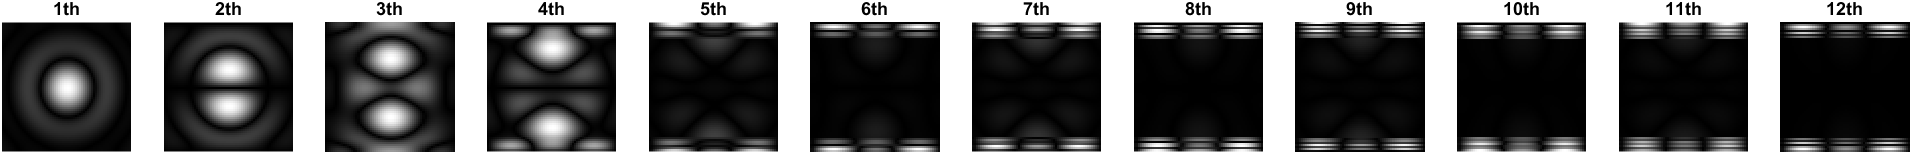
\includegraphics[width=0.8\linewidth]{../figures/ex_gu4_0.png}  
   %\caption{Ideal modes}
    \label{fig:modes_u}
 \end{subfigure}
 \begin{subfigure}{1\textwidth}
    \centering
    % include second image
    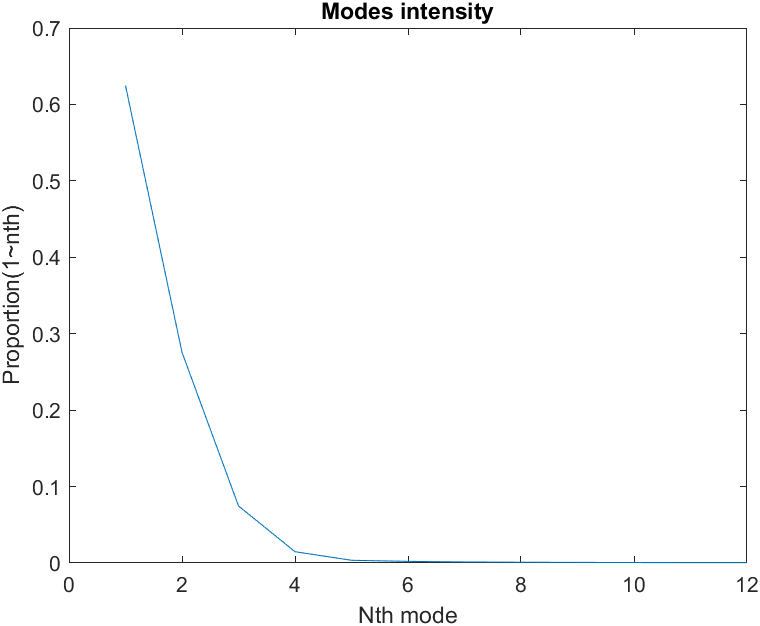
\includegraphics[width=.4\linewidth]{../figures/ex_gu4_0_s.png}  
    %\caption{Put your sub-caption here}
    %\caption{Singular value distribution}
    \label{fig:modes_u_phaze}
 \end{subfigure}
 \end{figure}
\end{frame}

\begin{frame} \frametitle{Example: Motion $\kappa$ (len=20,theta=45)}
\begin{figure}[H]
\centering
\begin{subfigure}{1\textwidth}
    \centering
    % include first image
    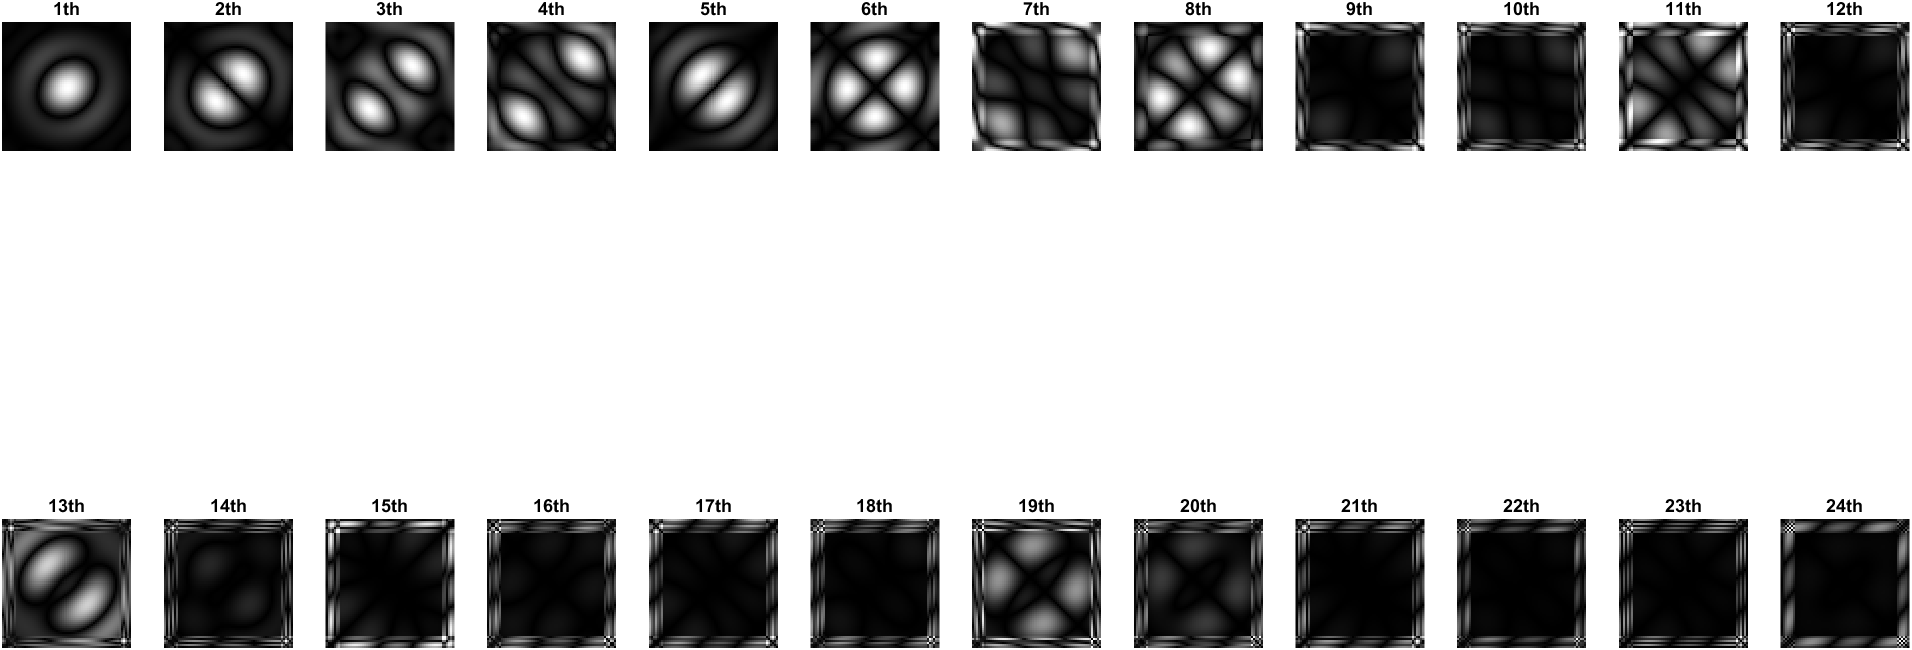
\includegraphics[width=0.8\linewidth]{../figures/ex_motion.png}  
   %\caption{Ideal modes}
    \label{fig:modes_u}
 \end{subfigure}
 \begin{subfigure}{1\textwidth}
    \centering
    % include second image
    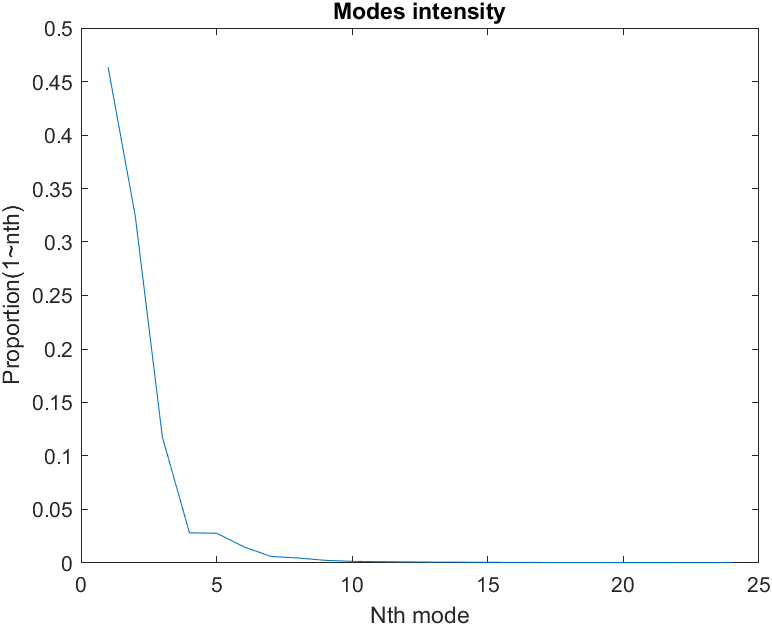
\includegraphics[width=.4\linewidth]{../figures/ex_motion_s.png}  
    %\caption{Put your sub-caption here}
    %\caption{Singular value distribution}
    \label{fig:modes_u_phaze}
 \end{subfigure}
 \end{figure}
\end{frame}



%\begin{frame} \frametitle{}
%\centering
%
%\end{frame}
\begin{frame} 

\centerline{\huge Thanks!}
\end{frame}

\end{document}
